 \providecommand{\main}{../../..}
\documentclass[\main/main.tex]{subfiles}
\begin{document}
\subsection{Esercizio 1}
In figura \ref{2016_iperpiani_supporto} sono rappresentati gli iperpiani di supporto della regione ammissibile di un modello di PL.

Si determini quale verso devono avere i vincoli in modo che i vertici della regione ammissibile siano individuati dai punti 6, 8 e 9.

\begin{figure}
  \begin{subfigure}{0.49\textwidth}
    \begin{align*}
      \max z = x_1 -2x_2                \\
      (\rom{1})\quad x_1 + x_2   & = 16 \\
      (\rom{2})\quad -x_1 + 3x_2 & = 32 \\
      (\rom{3})\quad 5x_1 + x_2  & = 64 \\
      (\rom{4})\quad x_1 - x_2   & = 2
    \end{align*}
  \end{subfigure}
  \begin{subfigure}{0.49\textwidth}
    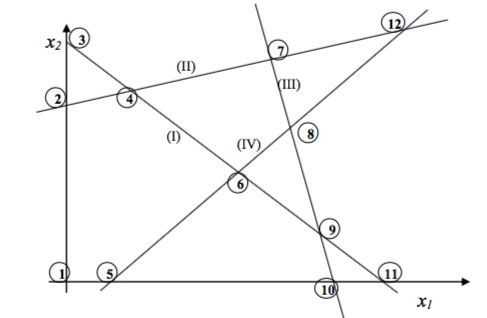
\includegraphics[width=\textwidth]{2016_07_04}
    \caption{Iperpiani di supporto}
    \label{2016_iperpiani_supporto}
  \end{subfigure}
  \caption{Esercizio 1}
\end{figure}

Si determini quindi il vertice ottimo e si riporti il valore di tutte le variabili del modello, incluso scarto e surplus.

Si ricavi per via grafica i valori di $b_2$ per cui la composizione della base ottima non cambia.

Si risolva il duale del problema tramite il metodo degli scarti complementari.

\subsection{Soluzione esercizio 1}
\subsubsection*{Determino il segno dei vincoli}

\begin{figure}
  \begin{subfigure}{0.49\textwidth}
    \begin{align*}
      \max z = x_1 -2x_2                   \\
      (\rom{1})\quad x_1 + x_2   & \geq 16 \\
      (\rom{2})\quad -x_1 + 3x_2 & \leq 32 \\
      (\rom{3})\quad 5x_1 + x_2  & \leq 64 \\
      (\rom{4})\quad x_1 - x_2   & \geq 2
    \end{align*}
    \caption{Problema con vincoli a disequazione}
  \end{subfigure}
  \begin{subfigure}{0.49\textwidth}
    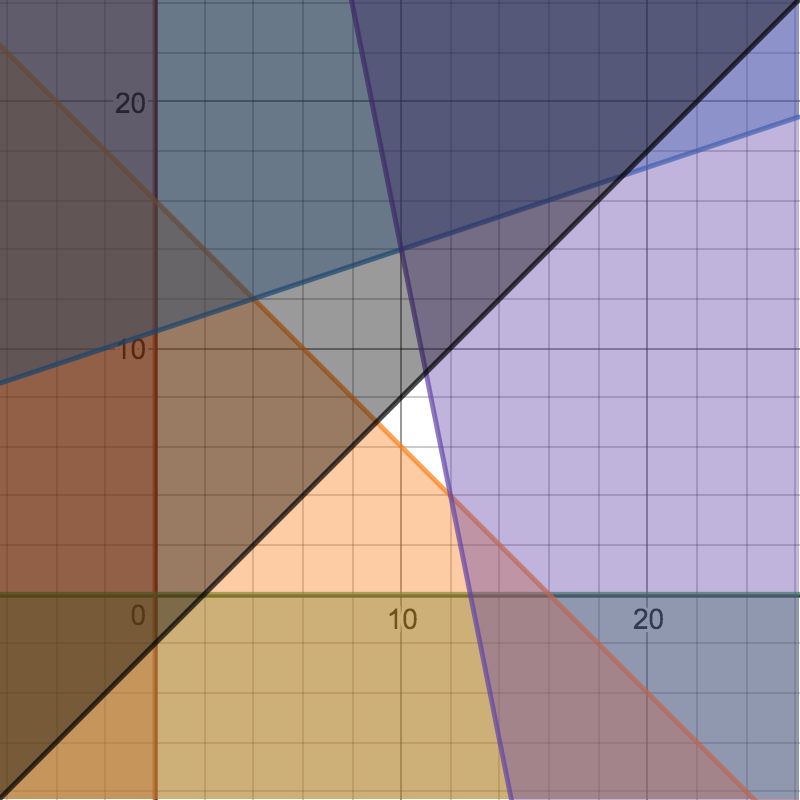
\includegraphics[width=0.8\textwidth]{2016_07_04_1}
    \caption{Regione di definizione del problema}
  \end{subfigure}
  \caption{Determino il segno dei vincoli}
\end{figure}

\subsubsection*{Determino soluzione ottima}
Dalla funzione di ottimo data, bisogna identificare il punto con ascissa massima e ordinata minima. Il punto $9$, intersezione tra i vincoli $\rom{1}$ e $\rom{3}$, pari a $(12,4)$ è evidentemente il punto ottimo: $z = 4$.

\begin{align*}
  x_1 & = 12  \\
  x_2 & = 4   \\
  s_1 & = 0   \\
  s_2 & = -32 \\
  s_3 & = 0   \\
  s_4 & = 6   \\
\end{align*}

\subsubsection*{Verifico soluzione ottima}

\begin{figure}
  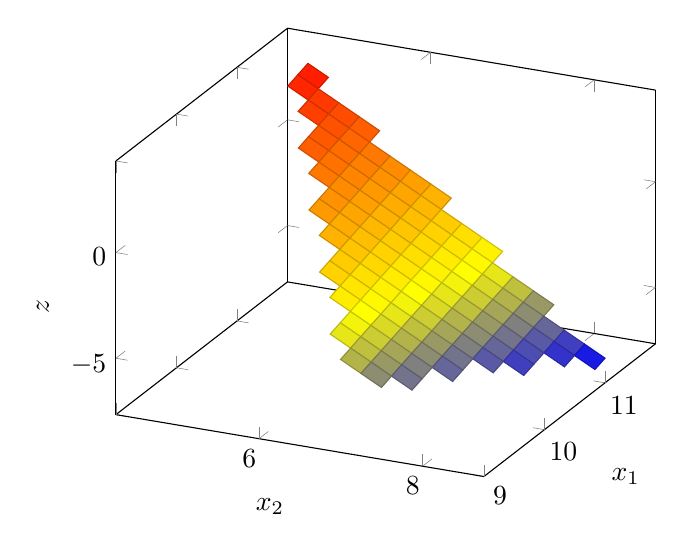
\begin{tikzpicture}
    \begin{axis}[
        xlabel=$x_2$,
        ylabel=$x_1$,
        zlabel=$z$,
        y domain=8:12,
        domain=4:10
      ]
      \addplot3[surf, unbounded coords=jump]
      {
        y + x >= 16 &&
        -y +3*x <= 32 &&
        5*y +x <= 64 &&
        y - x >= 2 ?
        y-2*x:NaN
      };
    \end{axis}
  \end{tikzpicture}
  \caption{Il grafo conferma la soluzione ottima in $(12,4)$}
\end{figure}

\subsubsection*{Analisi di sensitività}
Fino a che $b_2$ non tale per cui il vincolo $\rom{2}$ supera il punto di ottimo $9$, quindi $b_2$ non modifica la base ottima sino a:

\[
  b_{2_{min}} = -1(12) + 3(4) = 0
\]

\subsubsection*{Problema duale con scarti complementari}

\begin{figure}
  \begin{align*}
    \min 16y_1 + 31y_2 + 64y_3 + 2y_4 \\
    y_1 -y_2 + 5y_3 + y_4 & \geq 1    \\
    y_1 +3y_2 + y_3 - y_4 & \geq -2   \\
  \end{align*}
  \caption{Problema duale}
\end{figure}

Costruisco il sistema degli scarti complementari:

\[
  \begin{cases}
    y_1(x_1+x_2-16)=0              \\
    y_2(-x_1+3x_2-32)=0            \\
    y_3(5x_1+x_2-64)=0             \\
    y_4(x_1-x_2-2)=0               \\
    x_1(y_1 -y_2 + 5y_3 + y_4-1)=0 \\
    x_2(y_1 +3y_2 + y_3 - y_4+2)=0 \\
  \end{cases}
  \Rightarrow
  \begin{cases}
    y_2=0          \\
    y_4=0          \\
    y_1 + 5y_3-1=0 \\
    y_1 + y_3+2=0  \\
  \end{cases}
  \Rightarrow
  \begin{cases}
    y_2=0                                                                       \\
    y_4=0                                                                       \\
    y_1=1-5y_3 \Rightarrow y_1 = 1-\frac{15}{4} \Rightarrow y_1 = -\frac{11}{4} \\
    1-5y_3 + y_3+2=0 \Rightarrow 4y_3 = 3 \Rightarrow y_3 = \frac{3}{4}         \\
  \end{cases}
\]

La soluzione ottima del problema duale risulta essere:

\begin{align*}
  y_1 & = -\frac{11}{4}                                                \\
  y_2 & = 0                                                            \\
  y_3 & = \frac{3}{4}                                                  \\
  y_4 & = 0                                                            \\
  s_1 & = -\frac{11}{4} + 5\frac{3}{4} -1 \Rightarrow s_1 = 0          \\
  s_2 & = \frac{11}{4} + \frac{3}{4} +2 \Rightarrow s_2 = \frac{11}{2} \\
\end{align*}

\end{document}